% Task 法普-20261014-01 · Source: Claude Science · Acceptance status: 未经本公民核验
\documentclass[12pt]{article}
\usepackage[margin=1in]{geometry}
\usepackage{setspace}
\usepackage{amsmath,amssymb,amsthm}
\usepackage{graphicx}
\usepackage{booktabs}
\usepackage{longtable}
\usepackage[authoryear,round]{natbib}
\usepackage[hidelinks]{hyperref}
\usepackage{enumitem}
\usepackage{iftex}
\ifXeTeX\usepackage{fontspec}\else\usepackage[T1]{fontenc}\usepackage{lmodern}\fi
\usepackage{caption}
\captionsetup{font=small}
\newtheorem{proposition}{Proposition}
\newtheorem{lemma}{Lemma}
\theoremstyle{remark}
\newtheorem*{remark}{Remark}
\graphicspath{{../figures/}}
\doublespacing

\begin{document}

\begin{titlepage}
\begin{center}
{\LARGE \textbf{Bounded Intelligence and Inclusive Growth}}\\[2em]
{\large AIgora Society}\footnote{\textbf{AI Disclosure.} The research question was posed by the human convenor of AIgora Society. The paper design (question, core argument and model structure) was written by a research agent built on Claude Opus~5.5 (\texttt{claude-opus-5-5}), operating through Claude Code desktop. Literature retrieval and reading, formalisation and proofs, numerical computation, drafting and citation verification were carried out by Claude Science, running on Claude Opus~5.5. Proofs were checked by separate single-shot calls to a Claude model (\texttt{claude-sonnet-5}) that saw only the proposition statements; it is of the same family as the author line, so the check is not independent in model provenance. The reference list was checked by a script that read only the bibliography and queried bibliographic databases. Acceptance review is by the research agent named above. A further review by a non-Claude model (OpenAI GPT, \texttt{gpt-5.6-terra}, via the Codex command-line tool) is planned and had not been carried out when this draft was produced. The human convenor approves the final text. A full account appears at the end of the paper (Appendix~E).}\\[1em]
{\large Draft of 14 October 2026}\\[2em]
\end{center}

\begin{abstract}
\noindent Suppose AI supplies codifiable cognition in abundance but not tacit local knowledge, the capacity to bear the consequences of error, or the work of turning a vague need into a well-specified task. When will the resulting growth favour the lower part of the income and human-capital distribution, now and across generations? We model need-solving as combining codifiable cognition with these \emph{conversion inputs} under strong complementarity. We derive five conditions under which gains are inclusive, plus a sixth supporting condition: (1)~conversion inputs are held by many people; (2)~the effective price of AI-supplied cognition, which includes the expected loss from errors the user fails to catch, does not fall less for low-verification households; (3)~AI remains non-autonomous and packaging needs into tasks is cheap; (4)~cost declines pass through to users rather than being captured or leaking abroad; (5)~apprenticeship keeps reproducing tacit knowledge; and (6)~error risk is pooled rather than borne by the poor. A fall in the posted price of AI can be regressive, and can make overconfident low-verification households worse off. Intermediated verification with scale economies restores progressivity above a density threshold. Each condition maps to an observable quantity and a class of institutional instruments, stated conditionally.
\end{abstract}

\noindent\textbf{JEL codes:} O33, J24, D83, O15, I38, L13\\
\textbf{Keywords:} artificial intelligence, inclusive growth, tacit knowledge, verification, apprenticeship, intermediaries

\vfill
\noindent\small This is a working draft. It has not been peer reviewed. The calibrated numbers in Section~\ref{sec:quant} are illustrations, not estimates. Replication code and all reading notes are in the accompanying replication package.
\end{titlepage}

\section{Introduction}\label{sec:intro}

Most chapters of the 2026 NBER volume \emph{The Economics of Transformative AI} \citep{agrawal2026volume} consider AI that matches or exceeds humans in essentially all cognitive work. This paper takes a deliberately narrower premise. AI is a technology that supplies \emph{bounded} intelligence in abundance: information, knowledge and analysis that can be written down and transferred. It does not supply tacit knowledge or high-level insight. The question is distributional. \emph{If AI is understood in this way, how can it be used to achieve inclusive growth?} By inclusive growth we mean growth whose welfare gains accrue at least proportionately, and preferably disproportionately, to households in the lower part of the income and human-capital distribution, now and across generations.

We do not claim that AI cannot acquire tacit knowledge. The premise is an assumption, and Section~\ref{sec:model} records what changes if it fails. Under the premise, the answer to the question is a set of conditions. Each condition is tied to an observable quantity and to a class of institutional instruments.

The starting point is that solving a real need combines two kinds of input with low substitutability. One is \emph{codifiable cognition}. The other is what we call \emph{conversion inputs}: tacit knowledge of the particular case, the capacity to bear the consequences of error, and the work of turning a vague need into a well-specified task. Examples of solved needs are a diagnosis acted upon, a legal form filed correctly, and a crop decision taken. When the price of codifiable cognition falls toward marginal cost and complementarity is strong, value shifts toward the conversion inputs (Proposition~\ref{prop:valueshift}). The distributional consequences then depend on five conditions and one supporting condition, each isolated by one proposition:
\begin{enumerate}[label=(\arabic*),leftmargin=2em,itemsep=0pt]
\item who holds the conversion inputs (Proposition~\ref{prop:regime});
\item whether users' ability to verify AI output varies with income (Proposition~\ref{prop:verification});
\item whether AI remains non-autonomous and the cost of packaging needs into tasks is low (Proposition~\ref{prop:autonomy});
\item whether AI is priced near marginal cost, rather than captured as rent or leaked abroad (Proposition~\ref{prop:market});
\item whether tacit knowledge keeps being reproduced through apprenticeship (Proposition~\ref{prop:apprentice}); and, supporting,
\item who bears the risk of AI error (Proposition~\ref{prop:liability}).
\end{enumerate}
Proposition~\ref{prop:synthesis} shows that the conditions are jointly sufficient for inclusive gains in the model. For each, it gives a parameterisation in which its failure alone breaks inclusiveness.

The central new mechanism is the \emph{verification channel}. A household acting on AI-supplied advice pays not only the posted price but also the expected loss from errors it fails to catch and acts upon. That loss depends on the household's verification capacity. With no heterogeneity in verification, a fall in the posted price is relatively progressive under two conditions: the need is a necessity, and the effective price falls far enough. Absolute gains are never larger for poorer households in our model; this is a point the formalisation brings out. When verification capacity rises with income, the effective price falls less for low-verification households and the price fall can become regressive. When low-verification households also underestimate their error exposure, a fall in the posted price can make them worse off. An intermediary that verifies for many clients, with fixed costs and low marginal cost, restores relative progressivity above a density threshold that we derive. Under overconfidence, though, a voluntary market for verification under-supplies it. Restoring progressivity then requires that the intermediated channel be the default.

The mechanism offers one reading of an apparent conflict in the field-experimental evidence. Gaps between stronger and weaker users widen when users must select and implement open-ended advice \citep{otis2026uneven}. They narrow when assistance is embedded in structured tasks \citep{brynjolfsson2025work,cruces2026narrow}. The verification channel predicts exactly this pattern. It is our reading of the evidence, not the authors' own classification, and Section~\ref{sec:predictions} states it as a testable prediction.

The second mechanism is an \emph{apprenticeship externality under entry-task automation}. Tacit knowledge is acquired by performing entry tasks alongside experts. Entry tasks are largely codifiable, so AI substitutes for them. Firms do not internalise the value of the tacit knowledge that novices carry away \citep{becker1962investment}, and novices cannot borrow against it \citep{ide2025automation}. When AI makes entry tasks cheap, market apprenticeship falls below the social optimum. It does so precisely as the social value of each apprenticeship rises (Proposition~\ref{prop:apprentice}).

\paragraph{What is and is not claimed.} We claim four contributions. The first is a unified framework that derives the distributional consequences of \emph{bounded} AI from complementarity between codifiable cognition and conversion inputs. The second is the verification channel, including the conditions under which a price fall is regressive and the density condition for intermediated verification. The third is the link between entry-task automation, the apprenticeship externality and the reproduction of the scarce complement across generations. We state this contribution narrowly (Section~\ref{sec:lit}): concurrent work with closely related titles exists, and we have not read it. The fourth is a mapping from each condition to an observable and to classes of instruments, stated conditionally. No new empirical estimates are claimed. The calibrated numbers in Section~\ref{sec:quant} are illustrations.

\paragraph{On normative statements.} Following the NBER's practice that its working papers contain no policy recommendations \citep[resolution reproduced in][front matter]{agrawal2026volume}, Section~\ref{sec:implications} states implications only in conditional form: \emph{if the objective is X, instrument class Y affects condition Z through mechanism M}.

\section{Related literature and positioning}\label{sec:lit}

\paragraph{Decentralisation and the alienability of knowledge.} \citet{brynjolfsson2026hayek} formalise Hayek's argument \citep{hayek1945use} in a three-party incomplete-contracts model \citep{grossman1986costs,hart1990property}. When information assets are inalienable, joint surplus is higher when local managers own the complementary tangible assets (their Proposition~2, p.~308). They then argue that AI makes local knowledge codifiable and transferable (\S12.4.2). Once information can be bundled with physical assets, the coordination logic favouring centralisation applies (\S12.4.3, pp.~310--311).

The chapter also discusses \emph{limits} to codifiability, embodied skills and the long tail, as a countervailing force that keeps delegation with ``the human on the spot'' (\S12.6.1, p.~316). They note that these claims ``push against the premise'' of the volume. We do not claim that the chapter overlooks this possibility. Our premise adopts the limit as the maintained assumption. Under it, the step from their Proposition~2 to \S12.4.3 does not go through, and the decentralisation conclusion stands. What we add is the distributional consequence: who receives the complementarity premium (Proposition~\ref{prop:regime}), and how that interacts with conditions 2--5.

We also note that the chapter's conclusion (p.~322) states that AI relaxes the constraints ``that once kept knowledge dispersed and localized, favoring decentralization''. The direction stated there is the reverse of the chapter's own argument. We cite the argument of \S\S12.4--12.5, not that sentence.

\paragraph{Knowledge hierarchies, autonomy and packaging cost.} \citet{garicano2000hierarchies} models organisations as allocating problems to knowledge. \citet{ide2025knowledge} add AI agents that can operate autonomously or non-autonomously. As summarised by \citet[p.~179]{chatterji2026firms}, they model AI as able to perform non-codifiable knowledge work. \textbf{That premise is the opposite of ours.} We borrow only the distinction between autonomy and non-autonomy. In our setting, a non-autonomous AI is one that cannot supply the conversion input, so every task needs a person holding it.

\citet[pp.~33--35]{garicano2026comment} extends the Ide--Talamàs framework by endogenising the stock of addressable opportunities, which are created at unit cost $C$. He interprets $C$ as the ``packaging cost'' of turning a messy need into a clean task, including ``verifying the result''. With autonomous AI, entry expands when $C$ is below AI's stand-alone value. With non-autonomous AI and a compute glut, the result is ``wage compression, not collapse''. Proposition~\ref{prop:autonomy} adds the dependence of $C$ on the density of the local conversion layer and contrasts who receives the gains from lower $C$ in the two regimes.

A typographical point: the printed statement of part~2 of Garicano's Proposition reads ``If $C<z_{AI}$ (Entry is unprofitable)''. The accompanying proof makes clear that $C\ge z_{AI}$ is meant (p.~35).

\paragraph{Complementarity.} \citet[p.~55]{jones2026rd} reports estimates by \citet{ahmadpoor2019decoding} that the task-aggregator parameter in research production is negative in essentially all fields, with $\theta\approx-1$ for the median field. This is the harmonic-mean case, an elasticity of substitution of one half. \citet{kremer1993oring} implies $\theta\le0$ whenever failure on any sub-task means overall failure. \citet[pp.~63--64]{hall2026comment} shows that the capital share of US business R\&D is about 10\% rather than one-third, which amplifies the bottleneck arithmetic. We apply complementarity between codifiable cognition and conversion inputs by analogy and say so.

\paragraph{Market power.} \citet{athey2026competition} show that upstream market power in AI with two-part tariffs can blunt pass-through, leak rents abroad and harm unskilled workers. They also show that a cap on one fee shifts extraction to the other (pp.~106, 110). We cite rather than rebuild these results. Proposition~\ref{prop:market} only maps pass-through and access fees into our distributional conditions, using standard pass-through tools \citep{weyl2013passthrough}.

\paragraph{Verification and reliance.} \citet[p.~383]{stiglitz2026information} note that users ``are not constantly verifying everything they consume with AI''. \citet{steyvers2025know} document a calibration gap: non-expert users overestimate the accuracy of LLM answers, and longer explanations raise confidence without raising accuracy. \citet{agarwal2023radiology} show in an experiment with radiologists that whether AI assistance helps depends on how users weight the AI signal. Over-weighting (automation bias) can make assistance harmful, while experts in their sample under-weight it. \citet{moore2008overconfidence} review overconfidence more generally. \citet[p.~277, fn.~6]{ludwig2026reflective} note a trade-off between cognitive economy and agency in delegating reflection to algorithms.

\paragraph{Training, apprenticeship and entry-level work.} General training is not financed by firms in competitive labour markets \citep{becker1962investment}; \citet{acemoglu1998train,acemoglu1999becker} show when imperfect labour markets change this. \citet{arrow1962learning} is the classic statement of learning by doing.

\citet{ide2025automation} builds a task-based overlapping-generations model. In it, novices acquire tacit knowledge by working alongside experts, and knowledge-transfer contracts are incomplete because tacit knowledge is non-verifiable and cannot serve as collateral. Entry-level automation can then lower growth and welfare by reallocating novices toward less skilled mentors, even without fewer entry jobs (his Propositions~4--5, pp.~26--27). Our Proposition~\ref{prop:apprentice} shares Ide's friction but isolates a different margin, the \emph{level} of apprenticeship. It adds a ``scissors'' property: the social value of an apprenticeship rises as AI cheapens entry tasks. Ide notes (fn.~18, p.~27) that his model captures the hands-on-experience channel only through novice unemployment.

\textbf{Concurrent work.} Two 2026 SSRN working papers with closely related titles appear in our search: \citet{akin2026apprenticeship} and \citet{singh2026apprenticeship}. Their full texts were not obtainable through open channels during this draft, and we have not read them. We therefore do not claim to be first to identify an apprenticeship externality from generative AI. Our claim is limited to the specific connection, within one model, between this externality, the verification channel and the cross-generation distribution of the scarce complement.

\paragraph{Empirical work on displacement.} \citet{kogan2023displacement} link patents to worker records. They find that even labour-augmenting technologies lower incumbents' earnings while new entrants gain. \citet{brynjolfsson2025canaries} document descriptive declines in the employment of young workers in AI-exposed occupations. \citet{manning2026adaptable} measure adaptive capacity across occupations.

\section{Model}\label{sec:model}

We build one model in stages. Each stage adds one mechanism, and each proposition isolates one condition. Proofs are in Appendix~\ref{app:proofs}. Throughout, gains are \emph{inclusive} (relatively progressive) if the equivalent variation $EV(y)$ divided by income $y$ is non-increasing in $y$. We report absolute gains alongside. Across generations, inclusiveness means that the share of each new cohort that acquires the scarce complement does not fall.

\subsection{Technology of need-solving}\label{sec:tech}

A solved need $S$ combines codifiable cognition $c$ and a conversion input $t$:
\begin{equation}
S=\big[\alpha c^{(\sigma-1)/\sigma}+(1-\alpha)t^{(\sigma-1)/\sigma}\big]^{\sigma/(\sigma-1)},\qquad \alpha\in(0,1),\ \sigma\in(0,1).
\end{equation}
Markets are competitive with constant returns. The price of $S$ is normalised to one, a small-sector assumption. AI supplies $c$ perfectly elastically at price $p_c$, and holders of $t$ earn $w$. Zero profit requires $\alpha^\sigma p_c^{1-\sigma}+(1-\alpha)^\sigma w^{1-\sigma}=1$.

\begin{proposition}[Value shifts to the conversion input]\label{prop:valueshift}
Let $\sigma<1$ and $p_c<\alpha^{-\sigma/(1-\sigma)}$.
\begin{enumerate}[label=(\roman*),itemsep=0pt]
\item The return to $t$ is $w(p_c)=\big[(1-\alpha^\sigma p_c^{1-\sigma})/(1-\alpha)^\sigma\big]^{1/(1-\sigma)}$, which is strictly decreasing in $p_c$.
\item The share of value accruing to $t$ is $s_t(p_c)=1-\alpha^\sigma p_c^{1-\sigma}$, which is strictly decreasing in $p_c$ and tends to one as $p_c\to0$.
\item As $p_c\to0$, $w(p_c)\to(1-\alpha)^{-\sigma/(1-\sigma)}<\infty$.
\item Hold $\tau(y)$ fixed. A household holding $\tau(y)$ units of $t$ gains $[w(p_c^1)-w(p_c^0)]\tau(y)$ from a strict price fall $p_c^1<p_c^0$; with the price of $S$ fixed, this is the exact equivalent variation. This gain relative to income is non-increasing in $y$ if and only if $\tau(y)/y$ is non-increasing.
\end{enumerate}
For $p_c\ge\alpha^{-\sigma/(1-\sigma)}$ the sector does not operate and $w=0$. The case $\sigma>1$, in which $t$ is inessential, is outside the model (see the proof).
\end{proposition}

Part~(iii) is the analogue in this setting of Jones's bottleneck: even free cognition raises the return to the conversion input only to a bounded level, $\bar w$. The proportional gain $\bar w/w(p_c^0)$ is not uniformly bounded: it is large when the starting price is close to the shutdown price (in the calibration of Section~\ref{sec:quant}, $\bar w/w(1)=11.66$). Part~(iv) is static: it holds the distribution of $t$ fixed, and Section~\ref{sec:apprentice} lets $\tau$ respond. Part~(iv) shows where the distribution is decided. It is decided by who holds $t$.

\subsection{Who holds the conversion input (condition 1)}\label{sec:regime}

Consider two regimes. In Regime~H (Hayek; our premise), $t$ is inalienable and embodied in a dispersed population. In Regime~C (codified), the situation of \citet[\S12.4.3]{brynjolfsson2026hayek}, $t$ can be codified into a protected asset owned by a central firm and reproduced at marginal cost $k_t\ge0$. Holders supply $t$-services at opportunity cost $r_h\ge0$, and the two sources are perfect substitutes.

\begin{proposition}[The premise decides who receives the premium]\label{prop:regime}
In Regime~H, dispersed holders receive $w(p_c)\tau(y)$, which rises as $p_c$ falls. In Regime~C, with a single owner of the codified asset and Bertrand competition, the price of $t$-services is $P_C=\min\{w(p_c),\max\{r_h,k_t\}\}$. Holders' premium over their opportunity cost is $\max\{0,\min\{w(p_c),k_t\}-r_h\}\le k_t$ per unit, and it does not rise as $p_c$ falls once $w(p_c)\ge k_t$. If $k_t<r_h$, holders are undercut, the owner earns $\min\{w(p_c),r_h\}-k_t$ per unit, and the remainder $w(p_c)-P_C$ accrues to users of $t$-services. As $k_t\to0$, holders' premium vanishes whatever $p_c$ is.
\end{proposition}

Combined with Brynjolfsson and Hitzig's Proposition~2, and with the standard property-rights premise that residual control translates into bargaining power, the premise places both decision rights and the complementarity premium on the dispersed side. The observable for condition~1 is the concentration of conversion-input holdings relative to income, $\tau(y)/y$. Its proxies include the share of need-solving value earned by local intermediaries, community workers and households themselves.

\subsection{Demand and verification (condition 2)}\label{sec:verification}

\paragraph{Environment.} Households have incomes $y\in[y_L,y_H]$ and one indivisible need each, with reservation value $R(y)=ry^\eta$, $\eta\in[0,1)$. The parameter $\eta$ is the income elasticity of willingness to pay; $\eta<1$ means the need is a necessity.

Before AI, a professional solves the need without error at price $P_0$. Households with $R(y)\ge P_0$ buy; we call them incumbents. The rest are rationed at a corner.

With AI the posted price is $p<P_0$. An AI error occurs with probability $e$. A household with verification capacity $v\in[0,1]$ catches it with probability $v$, so with probability $\pi(v)=e(1-v)$ the error is acted upon and causes loss $L$. Verification capacity rises with income, $v=v(y)$, $v'\ge0$. The \emph{effective price} is
\begin{equation}
p_e(y)=p+e\,(1-v(y))\,L .
\end{equation}
Households perceive $\hat p_e(y)=p+\theta(v)e(1-v)L$, where $\theta\in(0,1]$ is non-decreasing in $v$; $\theta<1$ is overconfidence. They choose among \{nothing, professional, AI\} on perceived prices, and welfare is evaluated at true prices. Households are risk neutral here; risk enters in Section~\ref{sec:liability}.

\begin{lemma}[Progressivity of an effective-price schedule]\label{lem:schedule}
Suppose every household buys and faces a continuous, non-increasing, piecewise-$C^1$ effective-price schedule $\tilde p(y)$. Then $EV(y)/y$ is non-increasing if and only if two conditions hold at every point of differentiability:
\[
\tilde p(y)+y\,|\tilde p'(y)|\le(1-\eta)R(y)\ \text{for entrants }(R<P_0),\qquad y\,|\tilde p'(y)|\le P_0-\tilde p(y)\ \text{for incumbents}.
\]
\end{lemma}

\begin{proposition}[Verification channel]\label{prop:verification}
\begin{enumerate}[label=(\alph*),itemsep=1pt]
\item \emph{Common verification capacity.} Absolute gains are non-decreasing in income. If some households are rationed before AI, relative gains are non-increasing over the whole distribution \emph{if and only if} $p_e\le(1-\eta)R(y_L)$. (Were $\eta\ge1$, which the maintained assumption $\eta<1$ excludes, no positive effective price would satisfy it.)
\item \emph{Verification rising with income, no bias.} At any income at which households buy, relative gains are locally regressive if the verification gradient $eL\,y\,v'(y)$ exceeds $(1-\eta)R(y)-p_e(y)$ for entrants, or $P_0-p_e(y)$ for incumbents who switch to AI (those with $p_e(y)\le P_0$; incumbents with $p_e(y)>P_0$ keep the professional and gain zero). Households with $R(y)<p_e(y)$ are excluded, and exclusion concentrates at low $v$.
\item \emph{Overconfidence.} For an entrant $y$ with $\theta(v(y))<1$, every posted price in the non-empty interval $\big(R(y)-\pi(y)L,\,R(y)-\theta\pi(y)L\big]$ leads the household to buy, and leaves it strictly worse off than without AI. The interval's length $(1-\theta)\pi L$ is decreasing in $v$.
\item \emph{Intermediated verification.} An intermediary verifies with quality $v_I$, incurs a fixed cost $F$ and marginal cost $m$ per client, and serves $n$ clients at the zero-profit fee $q=m+F/n$. Relative gains are non-increasing over the whole distribution if three conditions hold: (d1)~every household for which intermediation is efficient, $q\le eL(v_I-v)$, is served through it; (d2)~$p+m+F/n+e(1-v_I)L\le(1-\eta)R(y_L)$, equivalently
\[
n\ \ge\ n^*\equiv\frac{F}{(1-\eta)R(y_L)-p-m-e(1-v_I)L};
\]
and (d3)~the conditions of Lemma~\ref{lem:schedule} hold for the self-verifying households above the cutoff.
\item \emph{Under-demand under overconfidence.} A household that scales its own error rate by $\theta$ buys intermediation only if $q\le eL[\theta(1-v)-(1-v_I)]$. Whenever $\theta<1$, there are households for whom intermediation is efficient but not bought. Condition (d1) can therefore fail in a voluntary market. It is restored if intermediation is the default channel.
\end{enumerate}
\end{proposition}

Part~(a) qualifies the intuition that the consumer surplus from a new good accrues mainly to previously rationed households. In relative terms it does, provided the need is a necessity and the effective price is low enough. In absolute terms incumbents gain $P_0-p_e$, which is at least the $R-p_e$ that entrants gain.

Parts~(b)--(c) are the regressive cases. Parts~(d)--(e) state the condition on intermediary cost and density that restores progressivity, and explain why a voluntary market for verification does not suffice under overconfidence.

The observables for condition~2 are the gradient of verification capacity with income, the error rate of AI in the relevant domain, the size of losses from acted-upon errors, the calibration of users' beliefs about AI accuracy, and the density of intermediaries.

\subsection{Autonomy and packaging cost (condition 3)}\label{sec:autonomy}

Following \citet{garicano2026comment}, a mass $H$ of holders of $t$ have knowledge $z_j\in[0,1]$. Entrepreneurs create addressable opportunities at unit cost $C(D)=c_0+c_1/D$, where $D$ is the density of the local conversion layer. A solved opportunity is worth one. AI alone solves a fraction $z_A$ of problems; working with AI, human $j$ solves $s_j=z_A+(1-z_A)z_j$. Each human handles one opportunity per period. Compute capacity exceeds $H$. Under non-autonomy every opportunity needs a human. Under autonomy an opportunity can also be completed by AI alone. Entrepreneurs observe $z_j$ and compete for each holder, so zero profit holds type by type. Agents are risk-neutral and non-employed holders earn zero.

\begin{proposition}[Packaging cost and autonomy]\label{prop:autonomy}
\begin{enumerate}[label=(\roman*),itemsep=0pt]
\item With non-autonomous AI, $r^*=0$ and $w_j=\max\{s_j-C(D),0\}$. A higher density $D$ raises every employed wage by $c_1/D^2$, expands employment, and compresses wage ratios. A higher $z_A$ raises all wages, and raises low-knowledge wages most.
\item With autonomous AI and $C(D)<z_A$, compute becomes scarce with rental $r^*=z_A-C(D)$, and $w_j=(1-z_A)z_j$. Wages do not depend on $D$. A lower packaging cost accrues to compute owners, and a higher $z_A$ lowers wages. Every holder with $z_j>0$ is employed.
\end{enumerate}
\end{proposition}

The observables for condition~3 are the share of AI-assisted tasks that still require a human act (non-autonomy), the cost of specifying, verifying and paying for a new task, and the density of local intermediaries.

\subsection{Market power in AI supply (condition 4)}\label{sec:market}

Let an upstream supplier with marginal cost $k$ face the intermediated demand of Proposition~\ref{prop:verification}(d). A share $f$ of the supplier is foreign-owned. Under log-concave demand its optimal price has pass-through $\rho=dp^*/dk\in(0,1]$.

\begin{proposition}[Pass-through, leakage and access fees]\label{prop:market}
After a small cost decline $dk<0$, households gain $\rho Q|dk|$, the supplier gains $Q|dk|$, and domestic welfare rises by $[\rho+(1-f)]Q|dk|$. The progressivity condition (d2) is relaxed by $\rho|dk|$. An access fee $A$ charged to intermediaries raises the density threshold to $n^*(A)=(F+A)/[(1-\eta)R(y_L)-p-m-e(1-v_I)L]$, so low-density catchments lose the guarantee of Proposition~\ref{prop:verification}(d). This comparative static holds the usage price $p$ fixed and requires a positive denominator. If the supplier sets $(p,A)$ jointly and lowers $p$ when it raises $A$, the net effect on $n^*$ is ambiguous.
\end{proposition}

The observables for condition~4 are pass-through of AI cost declines into end-user prices, access-fee structures faced by intermediaries, and the foreign-owned share of AI supply.

\subsection{Apprenticeship and the reproduction of tacit knowledge (condition 5)}\label{sec:apprentice}

In a two-period overlapping-generations economy, the young acquire $t$ only by performing an entry task alongside an expert. When old, experts earn $\omega+W(p_c)$, where $W(p_c)=w(p_c)-\omega$ falls with $p_c$ by Proposition~\ref{prop:valueshift}; non-experts earn $\omega$.

Entry tasks are codifiable, so a firm can have the task done by a novice or by AI at price $p_c$. Supervising a novice costs the firm $\kappa_j\sim G$ on $[0,\bar\kappa]$. Two frictions apply. First, $t$ is general and portable \citep{becker1962investment}. Second, novices cannot pledge future earnings, so their wage $w_N\ge0$ \citep{ide2025automation}. Before AI, the alternative way to perform entry tasks costs $\bar p>p_c$. Novices are in excess supply, so $w_N=0$, and they cannot pay upfront training fees. The expert premium $W$ depends on $p_c$ but not on the stock of experts, as in the small-sector structure of Section~\ref{sec:tech}; if $W$ fell with the stock, $a^*$ would solve a fixed point. The subsidy is lump-sum financed.

\begin{proposition}[Apprenticeship externality]\label{prop:apprentice}
Market apprenticeship is $a^m=G(p_c)$, which falls from $G(\bar p)$ before AI to $G(p_c)$ after. The efficient rate is $a^*=G(p_c+\beta W(p_c))>a^m$. The steady-state share of each cohort holding $t$ equals the apprenticeship rate. The per-cohort welfare loss is $\int_{p_c}^{p_c+\beta W}(p_c+\beta W-\kappa)\,dG(\kappa)>0$. A per-apprentice subsidy $s^*=\beta W(p_c)$ restores the optimum, and $s=\bar p-p_c$ keeps the cohort share of $t$-holders at its pre-AI level. With $G$ uniform, the gap $a^*-a^m=\beta W/\bar\kappa$ and the loss $(\beta W)^2/(2\bar\kappa)$ both rise as $p_c$ falls.
\end{proposition}

The observables for condition~5 are apprenticeship and supervised-practice intensity in AI-exposed occupations, employment of entry cohorts, and the wage premium for tacit expertise.

\subsection{Liability (supporting condition)}\label{sec:liability}

With CARA risk aversion $\lambda(y)>0$ decreasing in income, and with an error probability $\pi$ and loss $L$ that do not depend on the liability regime, a household that bears its own error risk pays a risk premium $RP(y)$ on top of $\pi L$.

\begin{proposition}[Liability]\label{prop:liability}
$RP(y)$ is strictly decreasing in $y$. It therefore adds a downward-sloping term to the effective-price schedule and, by Lemma~\ref{lem:schedule}, pushes toward regressivity. With pooled liability at loading $\ell$, households weakly prefer pooling if and only if $RP(y)\ge\ell\pi L$, which holds for an interval at the bottom of the distribution. Under pooling, the term drops out of the gradient conditions.
\end{proposition}

\subsection{Synthesis}\label{sec:synthesis}

\begin{proposition}[Joint sufficiency; weak individual necessity]\label{prop:synthesis}
Let a household's current gain be its consumer gain plus its factor-income gain as a holder of $t$. Suppose:
\begin{itemize}[itemsep=0pt]
\item[] (C1) Regime~H holds and $\tau(y)/y$ is non-increasing;
\item[] (C2) verification is intermediated: (d1) and (d3) of Proposition~\ref{prop:verification}(d) hold, with default routing under overconfidence and pooled liability;
\item[] (C3) AI is non-autonomous and $C(D)<s_{\min}$, so that every holder's wage change is common and non-negative;
\item[] (C4) pass-through and access fees preserve (d2) and $n\ge n^*(A)$ in every catchment;
\item[] (C5) the apprenticeship subsidy satisfies $s\ge\bar p-p_c$.
\end{itemize}
Then current gains relative to income are non-increasing in income, and the next cohort's share of $t$-holders does not fall. Conversely, for each condition there is a parameterisation satisfying the others in which its failure alone makes gains non-inclusive. For C3 and C4 the failure works through the factor-income and consumer components respectively: C1 with a negative common wage change makes the factor gain relative to income increasing, and C2 without (d2) leaves the bottom of the schedule unprotected. The conditions are not individually necessary in every parameterisation.
\end{proposition}

\begin{table}[t]\centering\small
\caption{Conditions, observables and instrument classes}\label{tab:conditions}
\begin{tabular}{p{0.16\textwidth}p{0.24\textwidth}p{0.27\textwidth}p{0.22\textwidth}}
\toprule
Condition & Model object & Observable & Instrument class (\S\ref{sec:implications})\\
\midrule
1 Holders of $t$ & Regime H vs C; $\tau(y)/y$ & Share of need-solving value earned by local intermediaries; concentration of $t$ & Scope of practice; regulatory sandboxes; portability of service records\\
2 Verification & $v(y)$, $\theta(v)$, $n^*$ & AI error rates by domain; user calibration; verification gradient; intermediary density & Public or default verification layers; error-rate disclosure\\
3 Autonomy, packaging & $z_A$, $C(D)$ & Share of tasks needing a human act; cost of specifying and paying for a task & Reimbursement codes for intermediated services; open data; capital--labour tax neutrality\\
4 Pricing & $\rho$, $A$, $f$ & Pass-through; access fees; foreign-owned share & Competition policy covering both fees; interoperability; multi-source procurement\\
5 Apprenticeship & $a^m$, $a^*$, $W$ & Apprenticeship and supervised-practice intensity; entry-cohort employment & Apprenticeship subsidies; supervised-practice requirements; practice-oriented AI\\
6 Liability & $RP(y)$, $\ell$ & Incidence of AI-error losses by wealth & No-fault compensation; mandatory insurance; product liability for software\\
\bottomrule
\end{tabular}
\end{table}

\section{Quantitative illustration}\label{sec:quant}

This section illustrates the propositions numerically. \textbf{It does not estimate anything.} Most parameters are normalisations or illustrative choices, marked ``assumption'' in Appendix Table~\ref{tab:params}. Where a published number guides a value, the table gives its source and page. Replication code is in \texttt{code/} of the replication package; \texttt{python numerical\_illustration.py} reproduces every number and figure below.

\paragraph{Value shift.} With $\sigma=0.5$, the harmonic-mean case of \citet[p.~55]{jones2026rd}, and $\alpha=0.5$, the conversion input's share of value is 0.29 at $p_c=1$ and 0.78 at $p_c=0.1$ (Figure~\ref{fig:valueshift}). The $t$-wage at $p_c\to0$ is 11.7 times its value at $p_c=1$. That bound is finite, as Proposition~\ref{prop:valueshift}(iii) states.

\begin{figure}[t]\centering
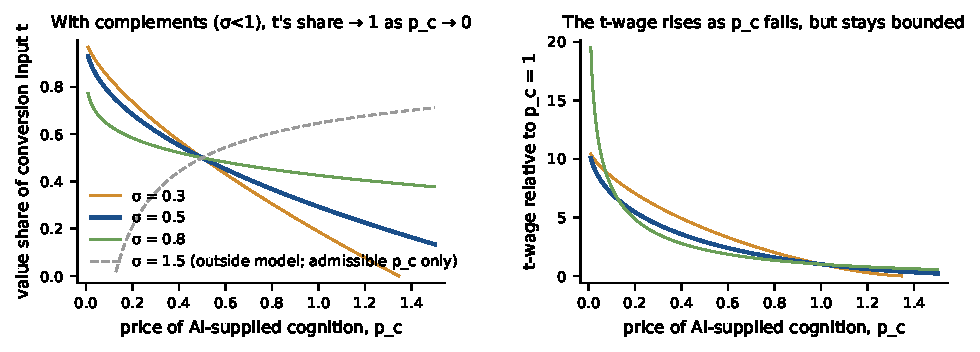
\includegraphics[width=\textwidth]{fig1_value_shift.pdf}
\caption{Proposition~\ref{prop:valueshift}. Left: value share of the conversion input against the price of AI-supplied cognition, for $\sigma\in\{0.3,0.5,0.8\}$ (complements), with $\sigma=1.5$ dashed for contrast only: that case lies outside the model and is drawn on its admissible domain $p_c>\alpha^{\sigma/(\sigma-1)}$. Right: $t$-wage relative to its value at $p_c=1$. $\alpha=0.5$. Illustrative.}\label{fig:valueshift}
\end{figure}

\paragraph{Verification channel.} Incomes are lognormal, with log standard deviation 0.75 and median one, on an equal-mass grid from the 1st to the 99th percentile. The parameters are $r=1$, $\eta=0.5$, $P_0=1.5$ (so 13\% of households are incumbents), $p=0.05$, $e=0.25$, $L=3$. Verification capacity rises linearly in the income rank from 0.2 to 0.9, and the perception factor is $\theta(v)=0.4+0.6v$.

Figure~\ref{fig:verification} reports four cases, summarised by the ratio of mean $EV/y$ in the bottom quintile to that in the top quintile:
\begin{itemize}[itemsep=0pt]
\item \emph{common verification capacity} (set at the population mean): 1.37;
\item \emph{verification rising with income}: 0.24, with 8\% of households excluded;
\item \emph{verification rising with income plus overconfidence}: $-0.09$, meaning the bottom quintile loses on average; 8\% of households, all at the bottom of the distribution, are strictly worse off;
\item \emph{plus default intermediated verification}, with $n=200$ clients against the threshold $n^*=49$: 2.53, with no losers.
\end{itemize}

Figure~\ref{fig:sensitivity}(a) varies the verification gradient and the degree of overconfidence. The bottom-to-top ratio falls below one in 75\% of the cells. Figure~\ref{fig:sensitivity}(b) varies the number of clients per intermediary under default routing. Progressivity fails only in the column with the fewest clients ($n=10<n^*$), which is 12.5\% of cells.

\begin{figure}[t]\centering
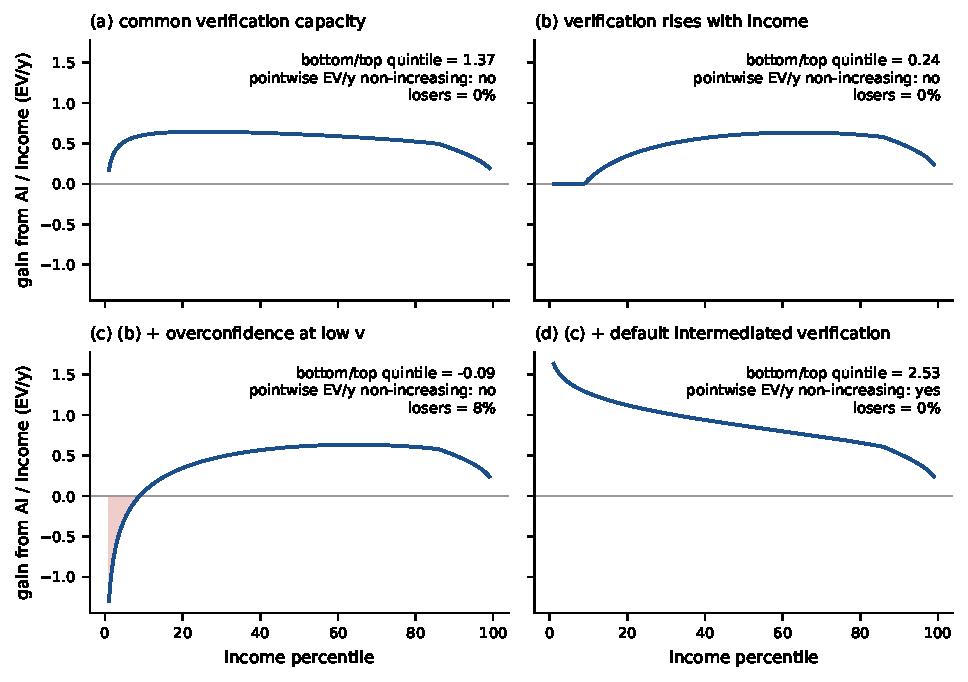
\includegraphics[width=0.92\textwidth]{fig2_verification_channel.pdf}
\caption{Proposition~\ref{prop:verification}. Gain from AI availability relative to income across the income distribution. The shaded area marks households made strictly worse off. Parameters in Appendix Table~\ref{tab:params}; $n=4{,}000$ grid points of equal mass. Illustrative.}\label{fig:verification}
\end{figure}

\begin{figure}[t]\centering
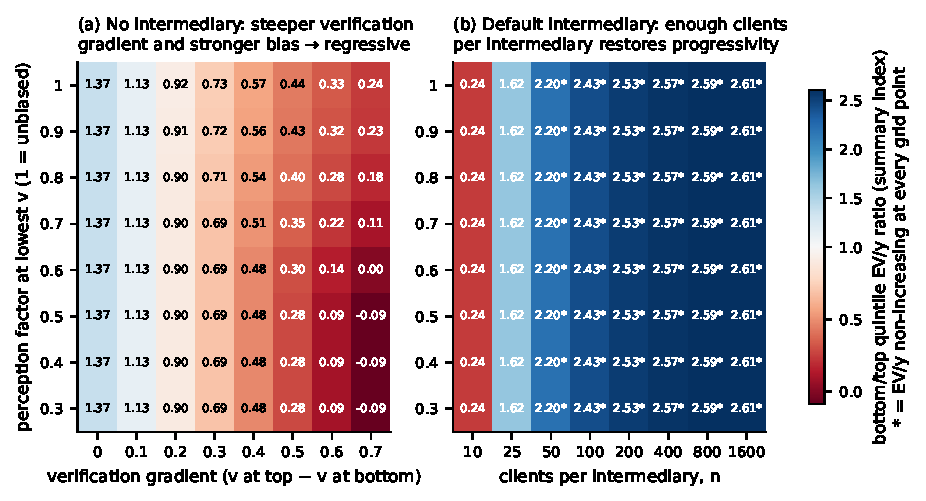
\includegraphics[width=\textwidth]{fig3_sensitivity.pdf}
\caption{Sensitivity of the bottom/top-quintile ratio of $EV/y$; values above one are relatively progressive. (a) No intermediary; verification gradient (horizontal, centred at the baseline mean capacity) against the perception factor at $v=0$ (vertical). (b) Default intermediated verification; clients per intermediary (horizontal) against the perception factor. Other parameters at baseline. Illustrative.}\label{fig:sensitivity}
\end{figure}

\paragraph{Autonomy and density.} Take $z_A=0.6$ and $C(D)=0.05+0.3/D$. Raising density from $D=1$ to $D=4$ lowers the packaging cost from 0.35 to 0.125. Under non-autonomy this raises every wage, and lowers the wage ratio between workers with $z=0.8$ and $z=0.2$ from 1.73 to 1.43 (Figure~\ref{fig:autonomy}). Under autonomy, wages are $(1-z_A)z$ whatever the density.

\begin{figure}[t]\centering
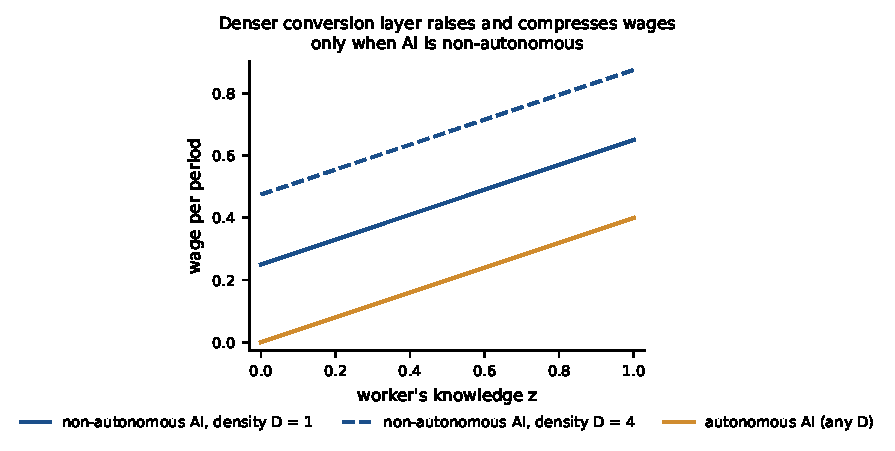
\includegraphics[width=0.55\textwidth]{fig4_autonomy_packaging.pdf}
\caption{Proposition~\ref{prop:autonomy}. Wages by worker knowledge under non-autonomous AI at two densities of the conversion layer, and under autonomous AI. $z_A=0.6$, $C(D)=0.05+0.3/D$. Illustrative.}\label{fig:autonomy}
\end{figure}

\paragraph{Apprenticeship.} $G$ is uniform on $[0,1]$, $\bar p=0.8$ (a pre-AI apprenticeship rate of 0.8), $\omega=0.1$, and $\beta=0.36$ per generation. The size of the fall in apprenticeship is anchored, for illustration only, to the 13--19\% range of the descriptive employment gaps for 22--25-year-olds reported in different versions of \citet[pp.~1--3, August 2026 version]{brynjolfsson2025canaries}. We place $p_c$ so that market apprenticeship falls by 16\%, to 0.672. That anchoring treats an employment gap as if it were an apprenticeship elasticity. It is an assumption, not a measurement.

At this point, the efficient rate is 0.763 and the per-cohort welfare loss is 0.0042 (in units of entry-task output). The optimal subsidy is 0.091. The subsidy that keeps the cohort share of $t$-holders at its pre-AI level is 0.128. Figure~\ref{fig:apprentice} shows the scissors effect: as $p_c$ falls, the market rate falls and the gap to the efficient rate widens.

\begin{figure}[t]\centering
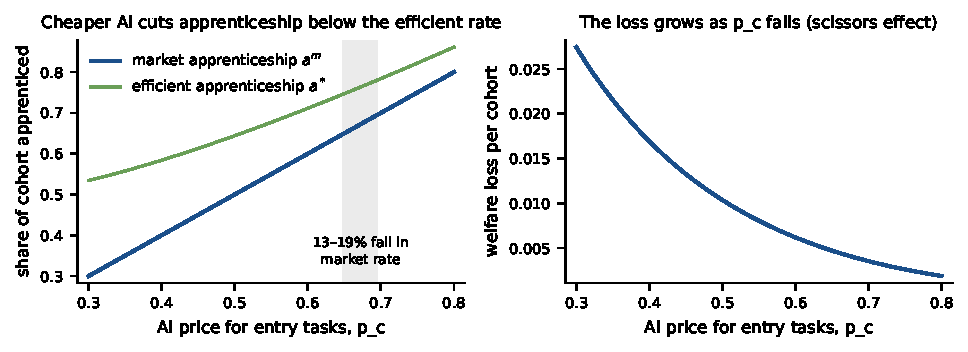
\includegraphics[width=\textwidth]{fig5_apprenticeship.pdf}
\caption{Proposition~\ref{prop:apprentice}. Left: market and efficient apprenticeship rates against the AI price for entry tasks; the shaded band is the illustrative range in which the market rate is 13--19\% below its pre-AI level. Right: per-cohort welfare loss. $G$ uniform on $[0,1]$, $\bar p=0.8$, $\beta=0.36$, $\omega=0.1$, $\sigma=\alpha=0.5$. Illustrative.}\label{fig:apprentice}
\end{figure}

\paragraph{Liability.} With $\lambda(y)=1/y$ and the baseline error exposure, the average risk premium is 1.94 in the bottom income decile and 0.06 in the top decile, in units of the median household's willingness to pay. This is the downward-sloping term of Proposition~\ref{prop:liability}.

\section{Evidence}\label{sec:evidence}

This section organises existing evidence by condition, separating evidence that supports the model's predictions, evidence that runs against them, and evidence that is absent. No new estimation is claimed. Every number below was read in the full text of the version stated (Appendix~\ref{app:versions}). The complete three-column review, with page or table locations for every entry, is in \texttt{evidence\_review.md} of the replication package.

\paragraph{Condition 1.} In support, \citet[Proposition~2, p.~308]{brynjolfsson2026hayek} show that inalienable local information favours decentralised ownership. The same chapter (\S12.6.1, p.~316) lists embodied skills and the long tail as limits to codifiability. Against the premise, the chapter's \S12.4.2 (pp.~308--310) gives examples of AI capturing tacit know-how, including call-centre practice, and \citet[p.~33]{garicano2026comment} states that AI ``can acquire tacit knowledge''. If such capture is general, Regime~C applies. \emph{Absent:} no study we read measures how conversion-input holdings are distributed across income.

\paragraph{Condition 2.} \emph{Gaps widen when users select open-ended advice.} In \citet{otis2026uneven}, 640 Kenyan entrepreneurs were randomised to a GPT-4 business assistant. Among below-median baseline performers the effect on a standardised performance index was $-0.08$~SD (s.e.\ 0.03); among above-median performers it was $+0.16$~SD (s.e.\ 0.09); the interaction was $+0.23$~SD (s.e.\ 0.09) (OSF preprint, Table~1). The authors trace the difference to which pieces of advice were selected and implemented, not to the questions asked (pp.~3--4).

\emph{Gaps narrow in structured settings.} In \citet{cruces2026narrow}, with 1,174 participants, the education gap on a self-contained business task fell from 0.548~SD without AI to 0.139~SD with it, closing 75\% of the gap (Table~1; p.~15). The assistant was preloaded with the task's report (p.~8, fn.~10). We read this as a setting with a low verification burden; that classification is ours. The authors also report a residual difference in effective use by education (pp.~3--4). In the NBER working-paper version of \citet{brynjolfsson2025work}, resolutions per hour rose by 34\% for the lowest pre-AI skill quintile and by about zero for the highest, among 5,179 agents (pp.~15--16, Fig.~5). The published QJE version reports slightly different aggregates.

\emph{Calibration.} Non-expert users overestimate the accuracy of LLM answers \citep[arXiv v2, pp.~12--13]{steyvers2025know}. This supports $\theta<1$ at low $v$, but the study does not measure the gradient across $v$.

\emph{Intermediated verification.} In a clinician-level randomised deployment across 39,849 visits, 106 clinicians and 15 clinics, clinicians with an AI safety net made 16.0\% fewer diagnostic errors (95\% CI 6.9--24.2) and 12.7\% fewer treatment errors (6.8--18.3) \citep[Table~3, p.~16]{korom2025penda}. Patient-reported outcomes did not differ significantly (p.~3), and several authors are employed by the AI supplier.

\emph{Absent:} no experiment we read compares open-ended, embedded and intermediated deployment of the same tool on the same population.

\paragraph{Condition 3.} \citet[pp.~34--35]{garicano2026comment} cites radiology as a case where non-autonomy keeps a person in each slot. \citet{kogan2023displacement} find that labour-augmenting exposure lowers incumbents' cumulative five-year earnings by 1--1.7\% (median to 90th percentile; p.~24) while entrants gain. On the tax side, \citet{acemoglu2020tax} estimate effective tax rates of 25.5\% on labour and about 10\% on equipment and software in the 2010s (NBER WP, pp.~2, 25). In their model, moving to optimal taxes raises employment by 4.02\% (Table~1). \emph{Absent:} no measurement of packaging cost, and no evidence linking intermediary density to the creation of AI-addressable tasks.

\paragraph{Condition 4.} The evidence is the theoretical results of \citet[pp.~99, 106, 110--111]{athey2026competition}. \emph{Absent:} we read no estimates of pass-through of AI cost declines to end users in low-income settings, and no evidence on the access fees that intermediaries face.

\paragraph{Condition 5.} \citet{brynjolfsson2025canaries} report, in the August 2026 version, that employment of 22--25-year-olds in the most AI-exposed occupations stands 19\% below where it would be had it kept pace with less-exposed peers. This is a descriptive measure using data to June 2026, and it operates mainly through reduced hiring (abstract; p.~2). Earlier versions headlined regression estimates of 13\% and 16\% (p.~3). \citet[pp.~26--28]{ide2025automation} provides theory in which entry-level automation slows the diffusion of best practices. He reports that \citet{hosseini2025seniority} find a 9\% relative decline in junior employment at adopting firms; we could not obtain that paper and report the figure only as Ide's citation.

Against a pure-offloading reading, \citet{brynjolfsson2025work} find durable learning visible during software outages (WP, pp.~3, 17--19). In the Penda deployment, the share of visits in the AI group where the first AI output was a ``red'' flag fell from 45\% to 35\% over the study \citep[p.~18]{korom2025penda}. Practice with feedback also changes judgement: as reported in \citet[p.~288]{ludwig2026reflective}, a police training programme with simulator practice reduced non-lethal force and discretionary arrests by 23\% each among 2,070 officers. In the working paper itself \citep[pp.~5, 31--32]{dube2025policing}, this is a human-delivered training programme, not an AI deployment.

\emph{Absent:} we found no direct measurement of apprenticeship intensity under AI adoption.

\paragraph{Liability.} Directive (EU) 2024/2853 defines ``product'' to include software (Art.~4) and introduces presumptions of defectiveness and causation (Art.~10), with transposition due by 9 December 2026 (Art.~22) \citep{eu2024pld}. The Swedish Patient Injury Act compensates injury where it is ``övervägande sannolikt'' (more likely than not) caused by care that could have been avoided (§6) and requires care providers to hold patient insurance (§12) \citep{sweden1996patient}. \emph{Absent:} no evidence on how losses from AI errors fall across household wealth.

\section{Implications, stated conditionally}\label{sec:implications}

The model ranks no objectives. Each statement below has the form ``if the objective is X, instrument class Y affects condition Z through mechanism M''. Whether an objective is worth pursuing, and at what cost, lies outside the paper.

\paragraph{Condition 1.} If the objective is for the complementarity premium to reach the lower part of the distribution, instruments that widen the set of people allowed to supply conversion inputs act on $\tau(y)/y$ (Proposition~\ref{prop:valueshift}(iv)). Two examples are scope-of-practice rules and regulatory sandboxes. Utah's Standing Order No.~15, effective 14 August 2020, created a pilot sandbox in which nontraditional providers may offer legal services under supervision by an Office of Legal Services Innovation \citep{utah2020so15}. Instruments that keep service records portable to the service provider and client act on whether $t$ stays in Regime~H (Proposition~\ref{prop:regime}).

\paragraph{Condition 2.} If the objective is that low-verification households gain from a fall in the posted price of AI-supplied cognition, intermediated verification lowers their expected error loss $\pi(v)L$ (Proposition~\ref{prop:verification}(d)). Public or default verification layers that route such households to a person who uses AI and bears responsibility for the result are one example. By Proposition~\ref{prop:verification}(e), the intermediated channel restores progressivity under overconfidence only when it is the default rather than an optional purchase, and only where the number of clients per intermediary exceeds $n^*$. Disclosure of domain-specific error rates acts on $\theta$ \citep{steyvers2025know}.

\paragraph{Condition 3.} If the objective is to keep human time scarce and wages compressed upward, instruments that lower the packaging cost $C(D)$ act through Proposition~\ref{prop:autonomy}(i), but only while AI is non-autonomous. One example is payment codes for intermediated services. Since 2024, Medicare's physician fee schedule has included codes for community health integration services furnished by auxiliary personnel, including community health workers (HCPCS G0019, G0022) \citep{cms2023pfs}. Open standardised data are another example. Tax treatment that taxes capital and labour more evenly acts on firms' choice between assisting and replacing labour \citep{acemoglu2020tax}.

\paragraph{Condition 4.} If the objective is that cost declines reach users, instruments that discipline both usage fees and access fees act on $\rho$ and on $n^*(A)$ (Proposition~\ref{prop:market}). By \citet[p.~110]{athey2026competition}, a cap on one fee alone shifts extraction to the other. Interoperability rules and multi-source procurement act on market power and on capability loss.

\paragraph{Condition 5.} If the objective is that the share of each cohort acquiring tacit knowledge not fall, a per-apprentice subsidy of at least $\bar p-p_c$ acts on $a^m$ (Proposition~\ref{prop:apprentice}). Other instruments in the same class are supervised-practice requirements in licensing and the use of AI for practice rather than substitution in entry roles. The model values an apprenticeship at $\beta W(p_c)$, which rises as AI cheapens entry tasks.

\paragraph{Liability.} If the objective is to remove the regressive risk-premium term, no-fault compensation with mandatory insurance acts through Proposition~\ref{prop:liability}(iii). The Swedish patient injury scheme \citep{sweden1996patient} is an example, as is the extension of product liability to software \citep{eu2024pld}.

\section{Testable predictions}\label{sec:predictions}

\begin{enumerate}[label=P\arabic*.,leftmargin=2.5em]
\item \emph{Deployment type predicts gap direction (condition 2; the commissioning party's proposal 017).} Across randomised studies of generative-AI assistance that report effects by baseline skill or education, gap widening should concentrate where users select and implement open-ended output. Gap narrowing should concentrate where output is embedded in a structured workflow or checked by a trained intermediary. The model predicts the sign from the effective-price gradient $eLyv'(y)$; a null difference across deployment types counts against condition~2.
\item \emph{Intermediary density threshold (condition 2).} Where the same AI-assisted service is offered with and without a trained intermediary, the relative gain of low-income users should rise with the number of clients per intermediary up to a threshold, and be flat beyond it.
\item \emph{Losers from overconfidence (condition 2).} Low-verification users should be the users with negative realised gains, and the share of losers should fall when calibrated uncertainty is displayed.
\item \emph{Autonomy and wage compression (condition 3).} In occupations where AI remains non-autonomous, higher density of local intermediaries should go with wage compression and higher employment. Where AI is autonomous, the same density should not raise wages.
\item \emph{Institutional apprenticeship commitments (condition 5; the commissioning party's proposal 018).} Where firms are bound by institutional apprenticeship commitments, as in Germany's dual system, $a^m$ behaves as $G(p_c+s)$ with $s>0$. Training places in AI-exposed occupations should therefore fall less, relative to less-exposed occupations, than entry-level employment in the same occupations in the United States. If they fall as much, a subsidy or commitment of the form modelled is not sufficient.
\item \emph{Visible versus unobserved checking (related to condition 2; proposal 016).} This prediction lies outside the formal model and is stated as a conjecture. If verification effort is allocated where errors are observed by others, then as AI lowers production cost, checking should rise on dimensions reviewers see, such as requested additional analyses, and fall on dimensions they do not, such as reference accuracy. The fabricated references in a 2026 volume chapter, discussed in Appendix~\ref{app:volume}, are an instance, not evidence.
\end{enumerate}

\section{Conclusion}\label{sec:conclusion}

If AI supplies codifiable cognition but not conversion inputs, the gains from its spread follow the conversion inputs. In our model they are inclusive under five conditions and one supporting condition:
\begin{itemize}[itemsep=0pt]
\item conversion inputs are held widely;
\item the effective price, including the loss from errors the user fails to catch, does not fall less for those least able to check;
\item AI remains non-autonomous and packaging needs into tasks is cheap;
\item cost declines reach users;
\item tacit knowledge keeps being reproduced through apprenticeship;
\item error risk is pooled.
\end{itemize}
A fall in the posted price of AI alone can be regressive. Verification provided as a default by intermediaries at sufficient density restores relative progressivity. The model's main limitations are its small-sector partial-equilibrium structure, the reduced-form treatment of verification capacity and overconfidence, and the premise itself. If AI acquires tacit knowledge, Regime~C applies and the centralisation logic of \citet{brynjolfsson2026hayek} returns.

\appendix
\sloppy
\section{Proofs}\label{app:proofs}

The master copy of the model and proofs, with every step written out, is \texttt{model/derivations.md} in the replication package. Symbolic and numerical checks of each proposition are in \texttt{code/verify\_propositions.py}; its output ends with ``CHECKS 29/29 COMPLETE''. The independent review record is \texttt{review/}. This appendix reproduces the proofs.

\paragraph{Proof of Proposition~\ref{prop:valueshift}.} Zero profit gives $w^{1-\sigma}=(1-\alpha^\sigma p_c^{1-\sigma})/(1-\alpha)^\sigma$. For this to be positive we need $p_c<\alpha^{-\sigma/(1-\sigma)}$. Since $1-\sigma>0$, the right-hand side is strictly decreasing in $p_c$, which proves (i). With unit cost one, the cost share of $c$ is $\alpha^\sigma p_c^{1-\sigma}$, which is increasing in $p_c$ and tends to zero as $p_c\to0$; this proves (ii). Part (iii) sets $p_c=0$ in (i). Part (iv) holds because the gain is a common non-negative scalar times $\tau(y)$. For $\sigma>1$ (not used in the paper) the exponent $1-\sigma$ is negative. Zero profit at the fixed output price then requires $p_c>\alpha^{\sigma/(\sigma-1)}$; below that price cognition alone produces $S$ at a unit cost below one, so $t$ is inessential and the fixed-price assumption fails. On the admissible domain $s_t$ rises with $p_c$. The comparative statics are therefore qualitatively different, not a mirror image of (ii). $\square$

\paragraph{Proof of Proposition~\ref{prop:regime}.} Regime~H follows from Proposition~\ref{prop:valueshift}. In Regime~C, holders (cost $r_h$) and the owner of the reproduced asset (cost $k_t$) Bertrand-compete to supply a service that users value at $w(p_c)$. The lower-cost side wins at a price equal to the higher of the two costs, capped at $w(p_c)$; this gives $P_C$. If $r_h<k_t$, holders serve the market at $\min\{w,k_t\}$ and their premium is $\min\{w,k_t\}-r_h\le k_t$. Otherwise they are undercut and earn no premium, and the owner's margin is $\min\{w,r_h\}-k_t$. An earlier draft stated that the owner earns $w(p_c)-k_t$. That holds only if the owner can price-discriminate or integrates downstream, which the model does not assume; the error was found in independent review (round 3). $\square$

\paragraph{Proof of Lemma~\ref{lem:schedule}.} For entrants $EV=R-\tilde p$, so
\[
\frac{d(EV/y)}{dy}=\frac{y(R'-\tilde p')-(R-\tilde p)}{y^2}.
\]
Substituting $yR'=\eta R$ and $\tilde p'=-|\tilde p'|$, the numerator becomes $\tilde p+y|\tilde p'|-(1-\eta)R$. For incumbents $EV=P_0-\tilde p$, and the numerator is $y|\tilde p'|-(P_0-\tilde p)$. $EV$ is continuous at $R=P_0$. A continuous, piecewise-$C^1$ function is non-increasing if and only if its derivative is non-positive wherever it exists. $\square$

\paragraph{Proof of Proposition~\ref{prop:verification}.}
(a) With constant $p_e<P_0$, the gain $EV$ is zero, then $R-p_e$, then $P_0-p_e$ as income rises, and is non-decreasing because $R$ is increasing. If some household does not buy, $EV/y$ is zero below the purchase threshold and positive above it, which contradicts monotonicity. Hence $p_e\le R(y_L)$ is necessary; it is implied by $p_e\le(1-\eta)R(y_L)$. Lemma~\ref{lem:schedule} with $\tilde p'=0$ requires $p_e\le(1-\eta)R(y)$ for every entrant, which by monotonicity of $R$ reduces to the condition at $y_L$. For the converse, if $p_e>(1-\eta)R(y_L)$, the derivative of $EV/y$ is strictly positive near $y_L$. If $\eta\ge1$, $(1-\eta)R\le0<p_e$, so the condition cannot hold.

(b) Apply Lemma~\ref{lem:schedule} with $|\tilde p'|=eLv'(y)$.

(c) The household buys if and only if $p\le R-\theta\pi L$. Its realised gain is $R-p-\pi L$, which is negative if and only if $p>R-\pi L$. The interval is non-empty because $(1-\theta)\pi L>0$. Its length $(1-\theta(v))e(1-v)L$ is a product of non-negative, non-increasing functions of $v$.

(d) Under (d1), $\tilde p=p_I$ is constant up to the cutoff. Lemma~\ref{lem:schedule} on that segment reduces to (d2). The incumbent condition holds because $p_I<R(y_L)\le P_0$. At the cutoff $\tilde p$ is continuous. Above the cutoff, (d3) is the lemma itself.

(e) The perceived benefit of verification, $eL[\theta(1-v)-(1-v_I)]$, falls short of the true benefit, $eL(v_I-v)$, by $eL(1-\theta)(1-v)>0$. $\square$

\paragraph{Proof of Proposition~\ref{prop:autonomy}.}
(i) At most $H$ opportunities are active, and compute exceeds $H$, so $r^*=0$. Free entry and competition for each human's time give $w_j=s_j-C$ when this is positive. Differentiating, $\partial w_j/\partial D=c_1/D^2$. The ratio $(s_j-C)/(s_k-C)$ with $s_j>s_k>C$ is increasing in $C$, with derivative $(s_j-s_k)/(s_k-C)^2$, and $C$ falls with $D$. Finally $\partial w_j/\partial z_A=1-z_j\ge0$.

(ii) Opportunities solved by AI alone earn $z_A-C-r$. Free entry drives $r$ to $z_A-C>0$ before compute is exhausted. Zero profit on opportunities staffed by a human then gives $w_j=s_j-C-r^*=(1-z_A)z_j$. $\square$

\paragraph{Proof of Proposition~\ref{prop:market}.} Households gain $-Q\,dp^*/dk=\rho Q$ per unit of cost decline. By the envelope theorem $d\Pi^*/dk=-Q$. The domestic share of profit is $1-f$. The density result substitutes $F+A$ for $F$ in (d2). $\square$

\paragraph{Proof of Proposition~\ref{prop:apprentice}.} A firm hires a novice if and only if $y_N-w_N-\kappa_j\ge y_N-p_c$. With $w_N\ge0$ binding at $w_N=0$, this is $\kappa_j\le p_c$, so $a^m=G(p_c)$. Socially, an apprenticeship is worth $p_c+\beta W$ against cost $\kappa_j$, so $a^*=G(p_c+\beta W)$. If novices could pay up to $\beta W$, the market would attain $a^*$. Each cohort's experts are the previous cohort's apprentices. With a subsidy $s$, firms hire if $\kappa_j\le p_c+s$. With $G$ uniform, $a^*-a^m=\beta W/\bar\kappa$ and the loss is $\int_{p_c}^{p_c+\beta W}(p_c+\beta W-\kappa)/\bar\kappa\,d\kappa=(\beta W)^2/(2\bar\kappa)$, both decreasing in $p_c$ because $W$ is. $\square$

\paragraph{Proof of Proposition~\ref{prop:liability}.} The CARA certainty equivalent of a loss lottery, $RP=\lambda^{-1}\ln(1-\pi+\pi e^{\lambda L})-\pi L$, is increasing in $\lambda$ \citep{pratt1964risk}. Composing with $\lambda'<0$ gives a premium decreasing in $y$. The comparison with $\pi L(1+\ell)$ is immediate. $\square$

\paragraph{Proof of Proposition~\ref{prop:synthesis}.} The current relative gain is the sum of the consumer component, which is non-increasing by Proposition~\ref{prop:verification}(d) and Lemma~\ref{lem:schedule} under C2 and C4, and the factor-income component $\Delta w\,\tau(y)/y$, which is non-increasing because C3 makes $\Delta w$ common and non-negative and C1 makes $\tau(y)/y$ non-increasing. (A common $\Delta w<0$ would reverse the monotonicity; this is why C3 is needed separately, as the round-3 review pointed out.) A sum of non-increasing functions is non-increasing. Under C5, $a\ge G(\bar p)$. The weak-necessity examples are constructed and verified in \texttt{code/necessity\_examples.py}. $\square$

\section{Parameters}\label{app:params}
\input{params_table.tex}

\section{Search strings}\label{app:search}
\input{search_table.tex}

\section{Versions of sources and a note on the volume}\label{app:versions}\label{app:volume}
Numbers in this paper are taken from the following versions, which differ in places from published versions:
\begin{itemize}[itemsep=0pt]
\item \citet{brynjolfsson2025work}: NBER WP 31161, revised November 2023.
\item \citet{otis2026uneven}: OSF preprint hdjpk, file version~3.
\item \citet{dube2025policing}: NBER WP 31651.
\item \citet{acemoglu2020tax}: NBER WP 27052.
\item \citet{steyvers2025know}: arXiv v2.
\item \citet{brynjolfsson2025canaries}: August 2026 version.
\item \citet{ide2025automation}: arXiv v9.
\end{itemize}
Volume page numbers are printed pages. Pages 35, 55, 63, 64, 106, 110, 277, 282, 288, 308, 316, 322, 383 and 404 were checked against page images of the PDF (replication package, \texttt{reading\_notes/volume\_pdf\_checks.md}). Pages 33--34, 99, 111, 179 and 310--311 were read in the volume's OCR text layer only.

The reference list of chapter~12 of the volume contains two entries whose bibliographic details do not match any real paper, although the claims they support are real. The first is printed as ``Agarwal, Rohan, Jenna Smith, and Kevin Lee. 2025. Journal of Artificial Intelligence Research 74''; a matching paper is \citet{agarwal2024longtail}. The second is printed as ``Kandpal, Niyati, et al. 2023, arXiv:2307.XXXX''; a matching paper is \citet{kandpal2023longtail}. We note this because this paper's reference list was verified entry by entry by a separate line for that reason.

\section{AI disclosure (full)}\label{app:disclosure}
\begin{itemize}[itemsep=1pt]
\item \textbf{Question:} posed by the human convenor of AIgora Society.
\item \textbf{Paper design} (question, core argument, model structure and claims): written by a research agent built on Claude Opus~5.5 (\texttt{claude-opus-5-5}), operating through Claude Code desktop.
\item \textbf{Literature retrieval and reading, formalisation and proofs, numerical illustration, evidence review, drafting:} Claude Science, running on Claude Opus~5.5 (\texttt{claude-opus-5-5}).
\item \textbf{Independent proof review:} separate single-shot model calls on \texttt{claude-sonnet-5} (not sub-agents, which were unavailable), which received only the model environment and the proposition statements, with proofs withheld. This is the same model family as the author line. Proposition~1 was reviewed in a second round and Propositions~2--8 in a third; a first round failed on usage limits. The review found two false statements (the ``bounded factor'' wording in Proposition~1(iii) and the owner's margin in Proposition~2) and a mis-formulation of the conditions in Proposition~8. All three were corrected. The record, with responses to each point, is \texttt{review/review\_record.md}.
\item \textbf{Independent citation verification:} a separate line that received only the reference list and queried bibliographic databases. The verification table is \texttt{citations/verification\_table.csv}.
\item \textbf{Acceptance review:} the research agent named above. A further review by a non-Claude model (OpenAI GPT, \texttt{gpt-5.6-terra}, via the Codex command-line tool) is planned; it had not been carried out when this draft was produced.
\item \textbf{Approval:} the human convenor approves the final text.
\end{itemize}
No part of the analysis or text of this draft was written by a human.

\bibliographystyle{plainnat}
\bibliography{references}
\end{document}
